\documentclass{article}
\usepackage{tikz}
\usepackage{fancyhdr}
\usepackage{extramarks}
\usepackage{pgfplots}
\usetikzlibrary{automata,positioning}
\usetikzlibrary{shapes.geometric, arrows}


\tikzstyle{startstop} = [rectangle, rounded corners, minimum width=3cm, minimum height=1cm,text centered, text width=3cm, draw=black, fill=red!30]
\tikzstyle{basicblock} = [rectangle, minimum width=3cm, minimum height=1cm,text centered, text width=3cm, draw=black, fill=blue!30]

\tikzstyle{io} = [trapezium, trapezium left angle=70, trapezium right angle=110, minimum width=3cm, minimum height=1cm, text centered, text width=2cm,draw=black, fill=blue!30]
\tikzstyle{process} = [rectangle, minimum width=3cm, minimum height=1cm, text centered, text width=2cm,draw=black, fill=orange!30]
\tikzstyle{decision} = [diamond, minimum width=3cm, minimum height=1cm, text centered, text width=2cm, draw=black, fill=green!30]



\tikzstyle{arrow} = [thick,->,>=stealth]
\begin{document}
	\large{}CAR LOGIC API OVERVIEW
	
	
	
	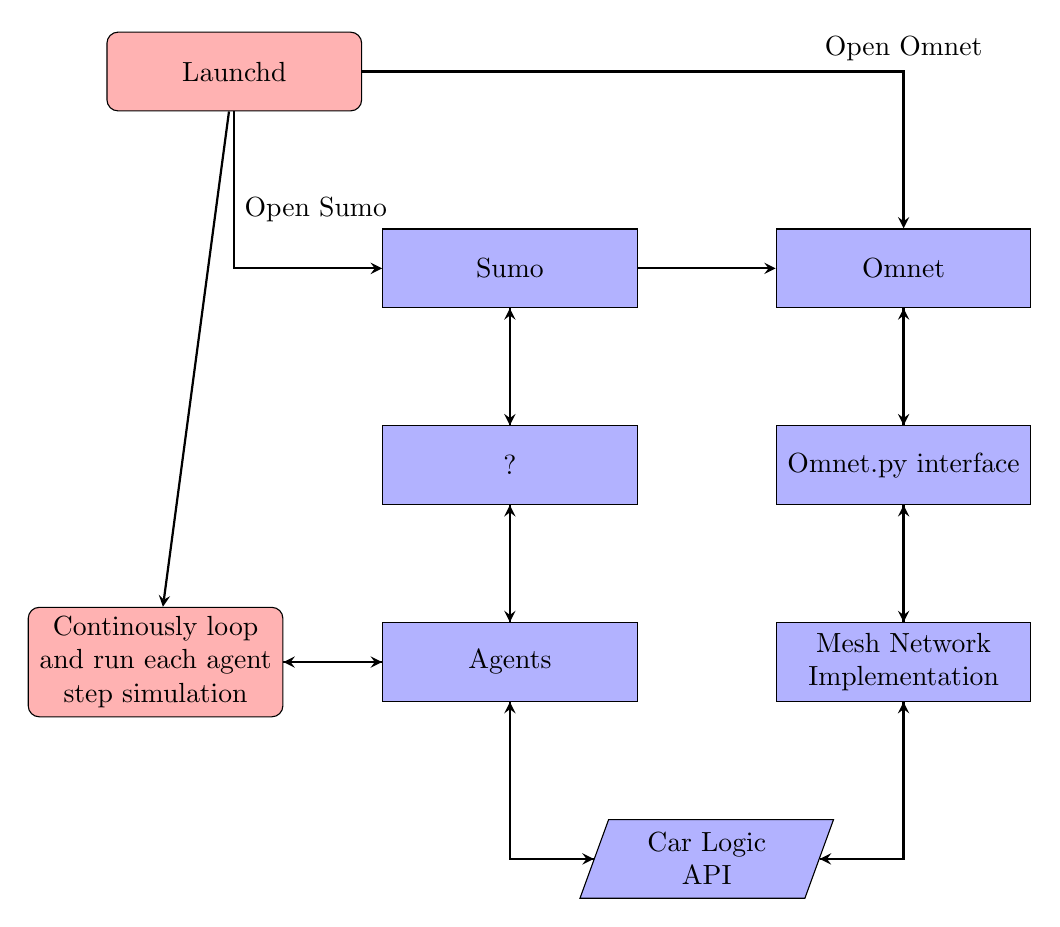
\begin{tikzpicture}[node distance=2.5cm]
	
	\node (launchd) [startstop, ] {Launchd};
	
	\node (sumo)[basicblock, below of=launchd, right of=launchd, xshift=1cm] {Sumo};
	
	\node (unknown)[basicblock, below of=sumo] {?};
	
	\node (agents) [basicblock, below of=unknown] {Agents};
	
	\node (carLogicAPI)[io, below of=agents, right of=agents]{Car Logic API};
	
	\node(meshNet)[basicblock, above of=carLogicAPI, right of=carLogicAPI]{Mesh Network Implementation};
	
	\node(omnetPY)[basicblock, above of=meshNet]{Omnet.py interface};
	
	\node(omnet)[basicblock, above of=omnetPY]{Omnet};
	
	\node(loopStatement)[startstop, left of=agents, xshift=-2cm]{Continously loop and run each agent\, step simulation};
	\draw [arrow] (loopStatement) -- (agents);
	\draw [arrow] (agents) -- (loopStatement);
	\draw [arrow] (launchd) -- (loopStatement);
	
	
	
	\draw [arrow] (launchd) |- node[anchor=west, yshift=.75cm]{Open Sumo} (sumo);
	\draw [arrow] (launchd) -| node [anchor=south]{Open Omnet}(omnet);
	
	\draw [arrow] (sumo) -- (omnet);
	\draw [arrow] (omnet) -- (omnetPY);
	\draw [arrow] (omnetPY) -- (meshNet);
	\draw [arrow] (meshNet) |- (carLogicAPI);
	\draw [arrow] (carLogicAPI) -| (agents);
	\draw [arrow] (agents) -- (unknown);
	\draw [arrow] (unknown) -- (sumo);
	
	\draw [arrow] (meshNet) -- (omnetPY);
	\draw [arrow] (omnetPY) -- (omnet);
	\draw [arrow] (agents) |- (carLogicAPI);
	\draw [arrow] (carLogicAPI) -| (meshNet);
	\draw [arrow] (sumo) -- (unknown);
	\draw [arrow] (unknown) -- (agents);
	\end{tikzpicture}
	
	\begin{enumerate}
		\item Launchd: Describe here 
		\item Sumo: Describe here 
		\item Omnet: Describe here 
		\item ?: Describe here 
		\item Omnet.py: Describe here 

		
	\end{enumerate}
\end{document}
